\section{Introduction}



Motion mimicking aims to find a policy to generate control signals for recovering demonstrated motion trajectories, which plays a fundamental role in physics-based character animation, and also serves as a prerequisite for many applications such as control stylization and skill composition. 
Although tremendous progress in motion mimicking has been witnessed in recent years, existing methods~\citep{peng2018deepmimic, peng2021amp} mostly adopt reinforcement learning (RL) schemes, which require alternatively learning a reward function and a control policy.
Consequently, RL-based methods often take tens of hours or even days to imitate one single motion sequence, making their scalability notoriously challenging.
In addition, RL-based motion mimicking highly relies on the quality of its designed ~\citep{peng2018deepmimic} or learned~\citep{peng2021amp} reward functions, which further burdens its generalization for complex real-world applications.




Recently, differential physics simulator (DPS) has achieved impressive results in many research fields, such as robot control~\citep{xu2022accelerated} and graphics~\citep{li2022diffcloth}.
Specifically, DPS treats physics operators as differentiable computational graphs, and therefore gradients from objectives (\textit{i.e.}, rewards) can be directly propagated through the environment dynamics to control policy functions.
Instead of alternatively learning between reward functions and control policies, the control policy learning tasks can be resolved in a straightforward and efficient optimization manner with the help of DPS. 
However, despite their analytical environment gradients, optimization with DPS could easily get into local optima, particularly in contact-rich physical systems that often yield stiff and discontinuous gradients~\citep{freeman2021brax, suh2022does, zhong2022differentiable}. 
Besides, numerical gradients could also vanish/explode along the backward path for long trajectories.






In this work, we propose DiffMimic, a fast and stable motion mimicking method with the help of DPS.
Different from RL-based methods that require heavy reward engineering and poor sample efficiency, DiffMimic reformulates motion mimicking as a state matching problem, which could directly minimize the distance between a rollout trajectory generated by the current learning policy and the demonstrated trajectory.
Thanks to the differentiable DPS dynamics, gradients of the trajectory distance can be directly propagated to optimize the control policy.
As a result, DiffMimic could significantly improve the sample efficiency with the first-order gradients.

However, simply utilizing DPS could not guarantee global optimal solutions.
In particular, the rollout trajectory tends to gradually deviate from the expert demonstration and could produce a large accumulative error for long motion sequences, due to the distributional shift between the learning policy and expert policy.
To address these problems, we introduce the \textit{\ourmethod{}} training strategy, which randomly inserts reference states into the rollout trajectory as anchor states to guide the exploration of the policy. 
Empirically, \ourmethod{} gives a smoother gradient estimation, which significantly stabilizes the policy learning of DiffMimic.


To the best of our knowledge, DiffMimic is the first to utilize DPS for motion mimicking. We show that DiffMimic outperforms several commonly used RL-based methods for motion mimicking on a variety of tasks with high accuracy, stability, and efficiency. In particular, DiffMimic allows learning a challenging \textit{Backflip} motion in only 10 minutes on a single V100 GPU.
In addition, we release the DiffMimic simulator as a standard benchmark to encourage future research for motion mimicking.

\begin{figure}[t]
    \centering
    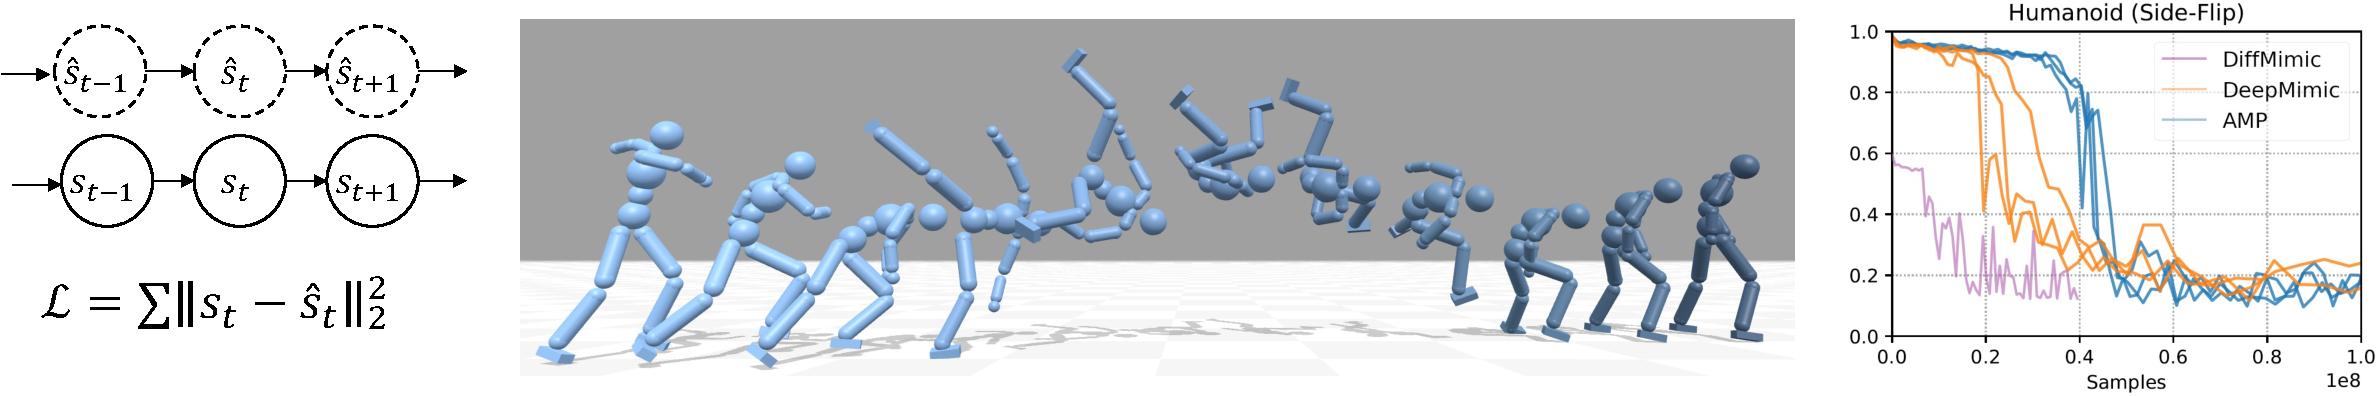
\includegraphics[width=\textwidth]{figures/teaser.pdf}
    \captionof{figure}{Overview of our method. \textbf{Left:} DiffMimic formulates motion mimicking as a straightforward state matching problem and uses analytical gradients to optimize it with off-the-shelf differentiable physics simulators. The formulation results in a simple optimization objective compared to heavy reward engineering in RL-based methods. \textbf{Middle:} DiffMimic is able to mimic highly dynamic skills, \eg, Side-Flip. \textbf{Right:} DiffMimic has a significantly better sample efficiency and time efficiency than state-of-the-art motion mimicking methods. Our approach usually achieves high-quality motion (pose error $<$ 0.15 meter) using less than $2\times10^7$ samples. }
    \label{fig:teaser}
\end{figure}